\documentclass[9pt,twocolumn,twoside]{pnas-new}
% Remove the twocolumn option to create a single column SI file if required. 
% Use the lineno option to display guide line numbers if required.
% Note that the use of elements such as single-column equations
% may affect the guide line number alignment. 

\templatetype{pnassupportinginfo}

\title{PNAS Supporting Information Template}
\author{LeadAuthor et al.}

\doi{10.1073/pnas.XXXXXXXXXX}

% Set the LAST citation number from your
% manuscript here
\continuecitefrom{33}

% For references that are already cited in the
% main manuscript, need to override its number
% manually here, based on its number in the main
% paper. Then cite this reference in the SI with
% \citepalias.
\defcitealias{berard1994embedding}{2}

\begin{document}

\maketitle

\section*{Supporting Information (SI)}

The main text of the paper must stand on its own without the SI. Refer to SI in the manuscript at an appropriate point in the text. Identify each Supporting Information file. Each file type should be numbered beginning with 1 (e.g., Fig. S1 and Table S1). Authors are limited to no more than 10 SI files, not including movie files. Authors who place detailed materials and methods in SI must provide sufficient detail in the main text methods to enable a reader to follow the logic of the procedures and results and also must reference the online methods. If a paper is fundamentally a study of a new method or technique, then the methods must be described completely in the main text. Because PNAS edits SI and composes it into a single PDF, authors must provide the following file formats only.

All Main and Supporting References should be included in the main text. PNAS now supports integrated references, and all supporting references should be included after the main text references in the main manuscript file. SI references should proceed numerically after the main text references (if the final main text reference is number 33, the first SI reference should be number 34). 

These are citations that only appears in the SI: \cite{varga2016multilingual} and \cite{olsen1992optimal}.
On the other hand, this is a citation to an earlier citation in the main manuscript: \citepalias{*berard1994embedding}. 
Mixing cites from main paper and SI within same bracket: (\citetalias{*berard1994embedding}, \citenum{olsen1992optimal}). And finally this is another SI citation \cite{baklouti2015towards}.

References in SI tables should also be included in the main reference section numbered by how it would appear once the SI is composed. If your SI is submitted as an Appendix (single PDF), SI references can remain in the combined SI file. 
\subsection*{SI Text}

Supply Word, RTF, or LaTeX files (LaTeX files must be accompanied by a PDF with the same file name for visual reference).

\subsection*{SI Figures}

Provide a brief legend for each supporting figure after the supporting text. Provide figure images in TIFF, EPS, high-resolution PDF, JPEG, or GIF format; figures may not be embedded in manuscript text. When saving TIFF files, use only LZW compression; do not use JPEG compression. Do not save figure numbers, legends, or author names as part of the image. Composite figures must be pre-assembled.

\begin{figure}[tbhp!]
\centering
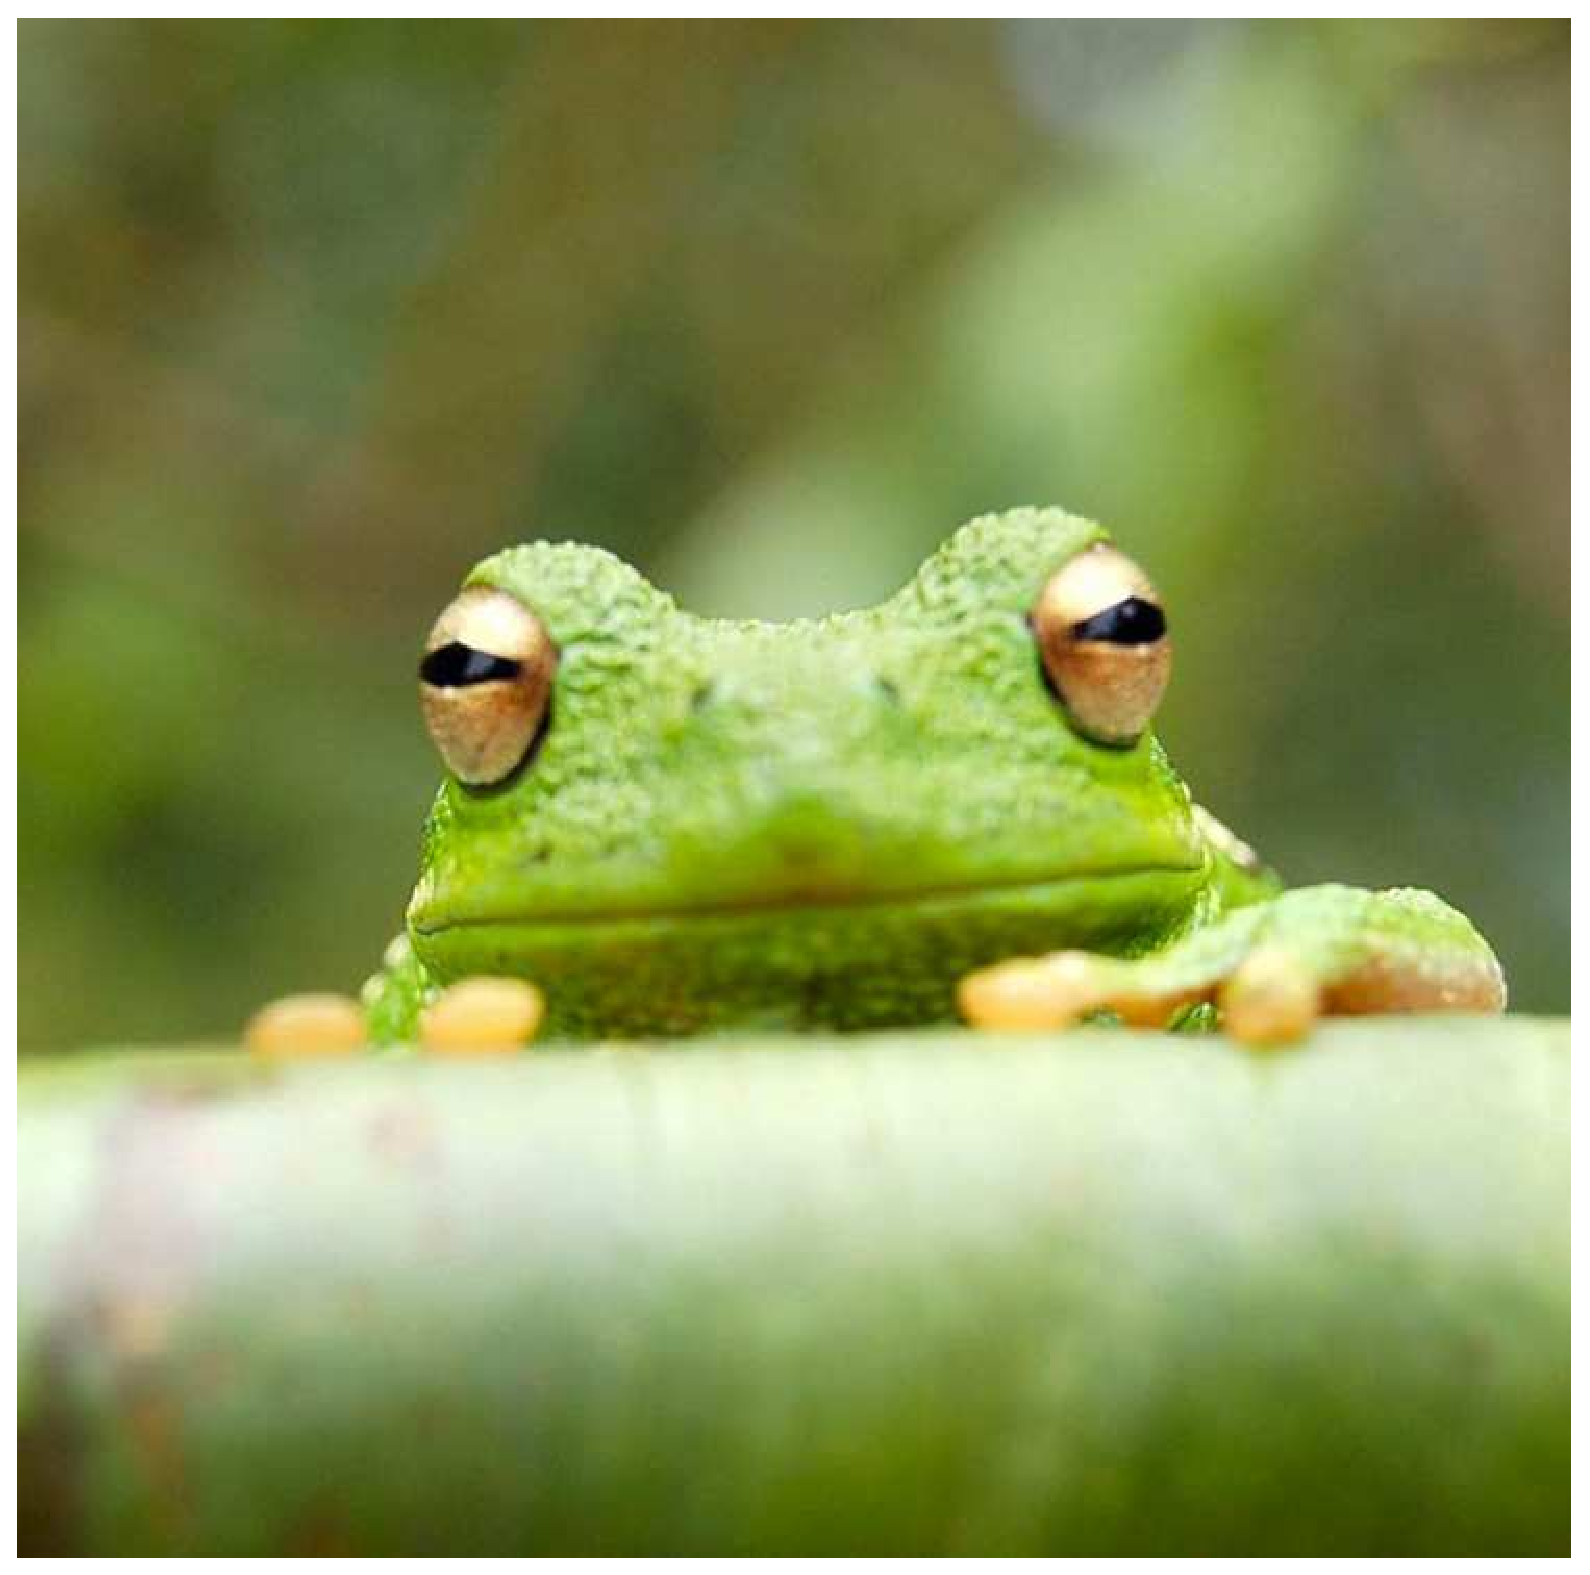
\includegraphics[width=.8\linewidth]{frog}
\caption{Placeholder image of a frog with a long example caption to show justification setting.}
\label{fig:frog}
\end{figure}

\begin{SCfigure*}[\sidecaptionrelwidth][t]
\centering
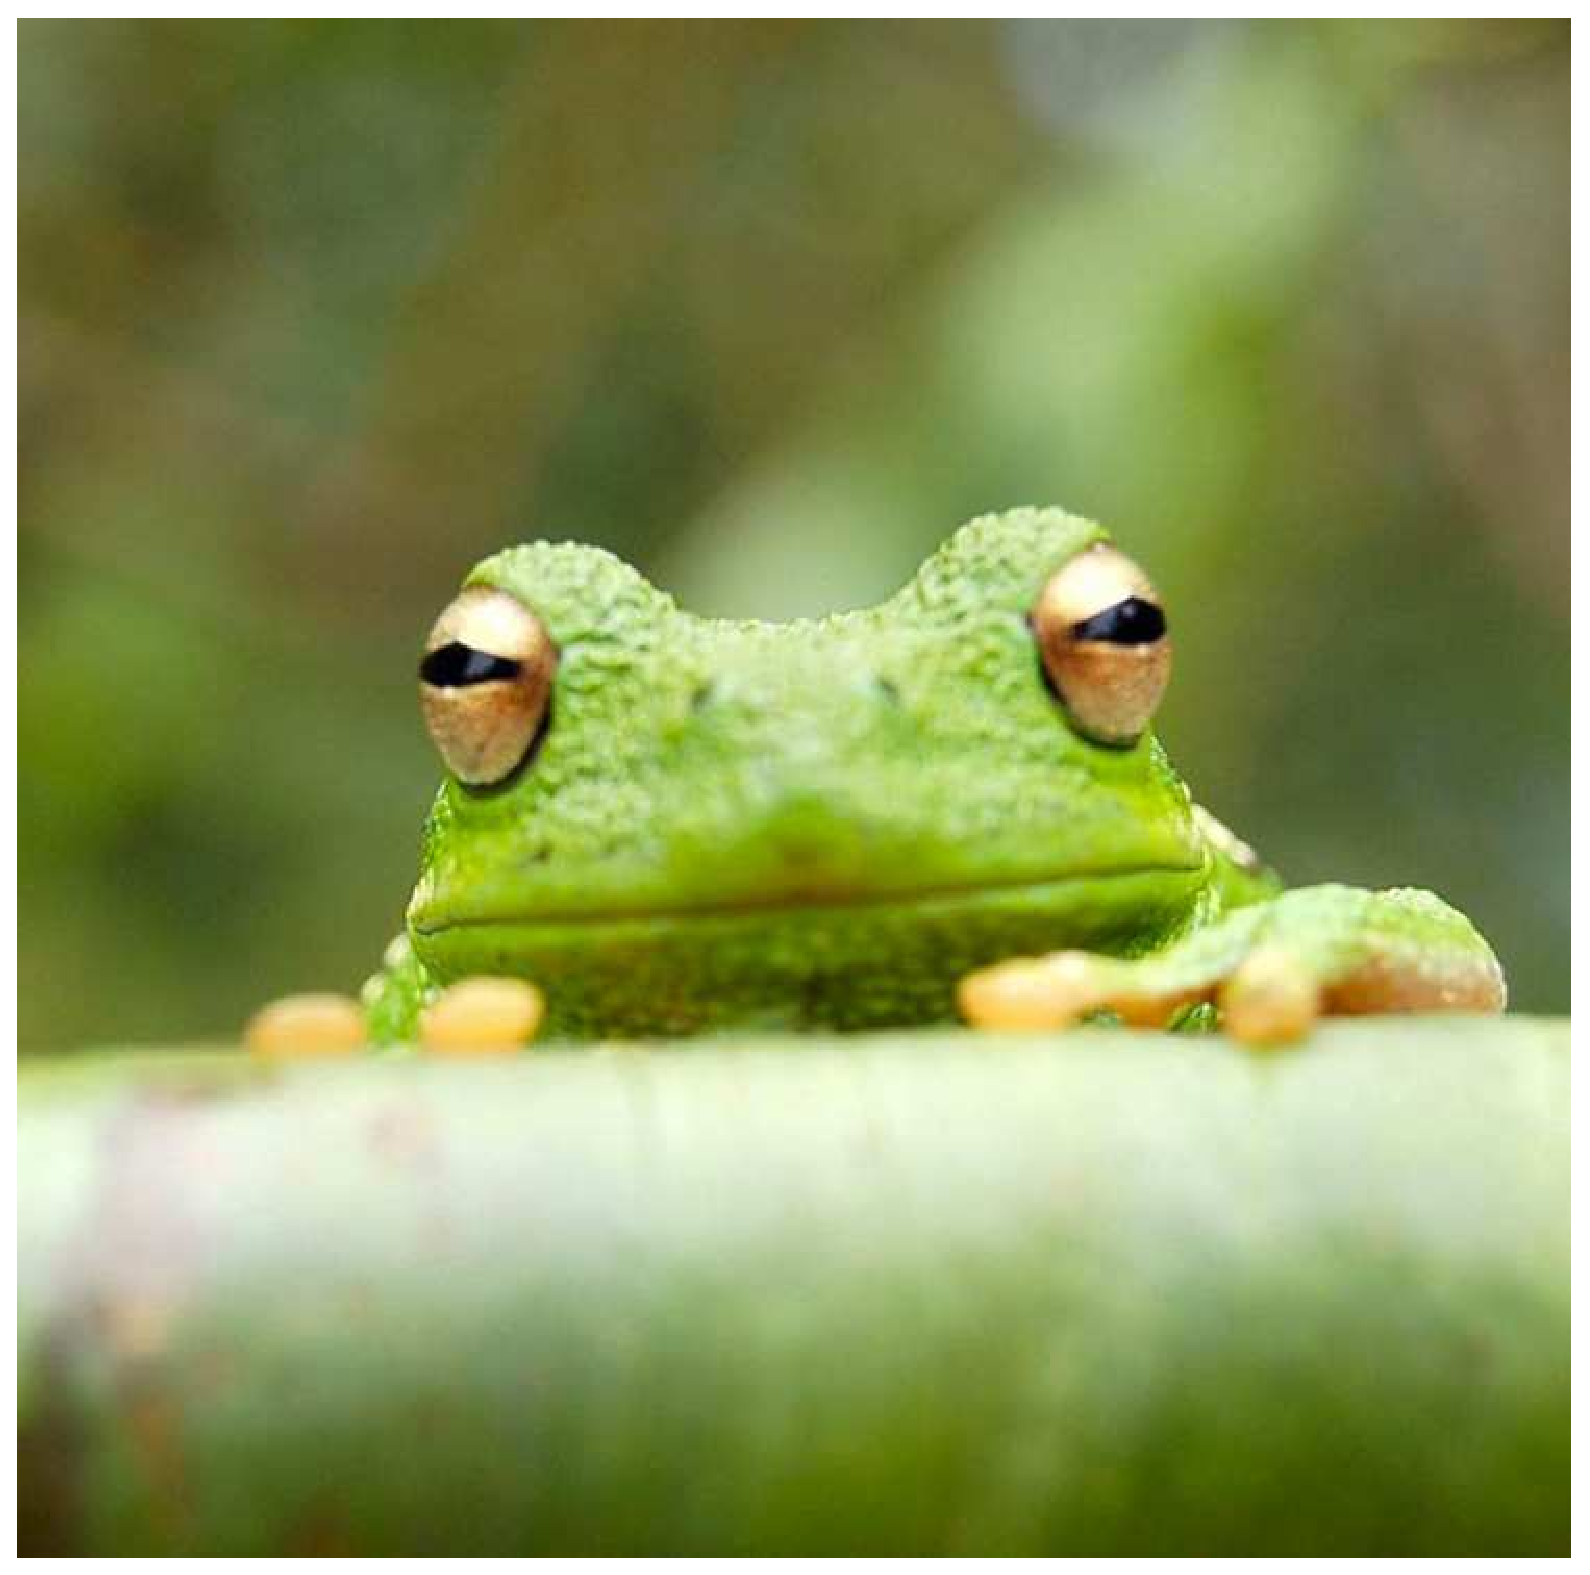
\includegraphics[width=11.4cm,height=11.4cm]{frog}
\caption{This caption would be placed at the side of the figure, rather than below it.}\label{fig:side}
\end{SCfigure*}


\subsection*{3D Figures}

Supply a composable U3D or PRC file so that it may be edited and composed. Authors may submit a PDF file but please note it will be published in raw format and will not be edited or composed.

\subsection*{SI Tables}

Supply Word, RTF, or LaTeX files (LaTeX files must be accompanied by a PDF with the same file name for visual reference); include only one table per file. Do not use tabs or spaces to separate columns in Word tables.

\begin{table}[tbhp!]
\centering
\caption{Comparison of the fitted potential energy surfaces and ab initio benchmark electronic energy calculations}
\begin{tabular}{lrrr}
Species & CBS & CV & G3 \\
\midrule
1. Acetaldehyde & 0.0 & 0.0 & 0.0 \\
2. Vinyl alcohol & 9.1 & 9.6 & 13.5 \\
3. Hydroxyethylidene & 50.8 & 51.2 & 54.0\\
\bottomrule
\end{tabular}

\addtabletext{nomenclature for the TSs refers to the numbered species in the table.}
\end{table}

\subsection*{SI Datasets}

Supply Excel (.xls), RTF, CSV, TXT, or PDF files. This file type will be published in raw format and will not be edited or composed. 

\subsection*{SI Movies}

Supply Audio Video Interleave (avi), Quicktime (mov), Windows Media (wmv), animated GIF (gif), or MPEG files and submit a brief legend for each movie in a Word or RTF file. All movies should be submitted at the desired reproduction size and length. Movies should be no more than 10 MB in size. 

\subsection*{Still images}

Authors must provide a still image from each video file. Supply TIFF, EPS, high-resolution PDF, JPEG, or GIF files. 

\subsection*{Appendices}

PNAS prefers that authors submit individual source files to ensure readability. If this is not possible, supply a single PDF file that contains all of the SI associated with the paper. This file type will be published in raw format and will not be edited or composed.

%% Important: use \nobibliography because references should NOT be printed in the SI. 
\nobibliography{pnas-sample}
%% Remember to list the cited references in your MAIN MANUSCRIPT  \nocite{key1,key2...} in the order that they are cited in this SI.

\end{document}